\section{Results}

\subsection{Data description}
\label{sec:agv_data_description}
Related and unrelated male and female samples from 3 different African populations were genotyped using the Illumina HumanOmni2.5 genotype chip array and sequenced on an Illumina HiSeq 2500 to different depths of coverage (table \ref{tab:samples}, figure \ref{fig:coverage}). The \gls{QC} of the samples genotyped on the Illumina HumanOmni2.5-4 and 2.5-8 platforms is described elsewhere\cite{Gurdasani2015} and on page \pageref{subsec:chipQC}.
% I need to figure out how to avoid this table from exceeding the page width.
%\begin{landscape}
%%%\begin{longtable}{lllllll}
\begin{table}[htp]
\centering
%\resizebox{\textwidth}{!}{%
\begin{tabular}{llrrllr}
\hline
Country & Ethnolinguistic group & Count & Depth & Source & Location & Size (TB) \\
\hline
%%%\endhead % all the lines above this will be repeated on every page
Uganda & Baganda & 1567 & 4x & UG2G & WTSI & 40.4 \\
Uganda & Banyarwanda & 199 & 4x & UG2G & WTSI & 5.1 \\
Uganda & Rwandese Ugandan & 76 & 4x & UG2G & WTSI & 1.9 \\
Uganda & Barundi & 51 & 4x & UG2G & WTSI & 1.4 \\
Uganda & Banyankole & 36 & 4x & UG2G & WTSI & 0.9 \\
Uganda & Bakiga & 30 & 4x & UG2G & WTSI & 0.8 \\
Uganda & Other & 41 & 4x & UG2G & WTSI & 1.1 \\
Uganda & Baganda & 100 & 4x & AGVP & WTSI & 2.7 \\
South Africa & Zulu & 100 & 4x & AGVP & WTSI & 2.3 \\
Ethiopia & Amhara & 24 & 8x & AGVP & WTSI & 1.0 \\
Ethiopia & Gumuz & 24 & 8x & AGVP & WTSI & 1.0 \\
Ethiopia & Oromo & 24 & 8x & AGVP & WTSI & 1.0 \\
Ethiopia & Somali & 24 & 8x & AGVP & WTSI & 1.0 \\
Ethiopia & Wolayta & 24 & 8x & AGVP & WTSI & 1.0 \\
Egypt & Unspecified & 100 & 8x & GDAP & WTSI & 5.0 \\
South Africa & Khoe-San (Nama) & 104 & 4x & GDAP & WTSI & 3.6 \\
%Uganda & Baganda & 3 & 30x & GDAP & WTSI \\
%South Africa & Zulu & 2 & 30x & GDAP & WTSI \\
%South Africa & Khoe-San (Nama) & 3 & 30x & GDAP & WTSI \\
%Chad & Northern and Southern & 100 & 30x & GDAP & WTSI \\
%Kenya & Kalenjin & 100 & 30x & GDAP & WTSI \\
%Nigeria & Igbo & 100 & 30x & GDAP & WTSI \\
%Ghana & Ashanti & 100 & 30x & GDAP & WTSI \\
%Morocco & Moroccans & 100 & 30x & GDAP & WTSI \\
%Burkina Faso & Gouin, Kaboro, Turka & 100 & 30x & GDAP & WTSI \\
%Gambia & Fula & 100 & 8x & MalariaGEN & ENA \\
Nigeria & Esan (ESN) & 99 & 4x & 1000G & 1000G & 2.2 \\
Gambia & Gambian (GWD) & 113 & 4x & 1000G & 1000G & 2.9 \\
Kenya & Luhya (LWK) & 101 & 4x & 1000G & 1000G & 2.2 \\
Sierra Leone & Mende (MSL) & 85 & 4x & 1000G & 1000G & 1.9 \\
Nigeria & Yoruba (YRI) & 109 & 4x & 1000G & 1000G & 2.3 \\
%Gambia & Gambian & 2 & 30x & 1000G & 1000G \\
%Nigeria & Esan & 2 & 30x & 1000G & 1000G \\
%Sierra Leone & Mende & 2 & 30x & 1000G & 1000G \\
%Kenya & Luhya & 2 & 30x & Coriell & Simons Foundation \\
%Kenya & Masai & 2 & 30x & Coriell & Simons Foundation \\
%Kenya & Luo & 2 & 30x & Geoge Ayodo & Simons Foundation \\
%Kenya & Somali & 1 & 30x & Geoge Ayodo & Simons Foundation \\
%Algeria & Mozabite & 8 & 8x & HGDP/Martin et al 2014 & NCBI-SRA \\
%DRC & Mbuti & 8 & 7x & HGDP/Martin et al 2014 & NCBI-SRA \\
%Namibia & San (Ju-hoan) & 6 & 10x & HGDP/Martin et al 2014 & NCBI-SRA \\
%Algeria & Mozabite & 2 & 30x & HGDP/Reich+Tyler-Smith & Simons Foundation and WTSI \\
%South Africa & Bantu (Tswana, Herero, Pedi, Sotho, Ovambo, Zulu) & 8 & 30x & HGDP/Reich+Tyler-Smith & Simons Foundation and WTSI \\
%South Africa & \begin{tabular}[b]{@{}l@{}}Bantu\\(Tswana, Herero, Pedi, Sotho, Ovambo, Zulu)\end{tabular} & 8 & 30x & HGDP/Reich+Tyler-Smith & Simons Foundation and WTSI \\
%Kenya & Bantu & 11 & 30x & HGDP/Reich+Tyler-Smith & Simons Foundation and WTSI \\
%CAR & Biaka Pygmy & 23 & 30x & HGDP/Reich+Tyler-Smith & Simons Foundation and WTSI \\
%Senegal & Mandenka & 22 & 30x & HGDP/Reich+Tyler-Smith & Simons Foundation and WTSI \\
%DRC & Mbuti Pygmy & 12 & 30x & HGDP/Reich+Tyler-Smith & Simons Foundation and WTSI \\
%Namibia & San (Ju-hoan) & 6 & 30x & HGDP/Reich+Tyler-Smith & Simons Foundation and WTSI \\
%Nigeria & Yoruba & 21 & 30x & HGDP/Reich+Tyler-Smith & Simons Foundation and WTSI \\
%South Africa & Khomani & 2 & 4x/9x & Kidd et al 2014 & NCBI-SRA \\
%South Africa & Khomani & 2 & 30x & Brenna Henn & Simons Foundation \\
%Sudan & Dinka & 3 & 30x & Michael Hammer & Simons Foundation \\
%Namibia & Khoisan & 1 & 10x & Schuster et al 2009 & NCBI-SRA \\
%South Africa & Xhosa/Tswana & 1 & 30x & Schuster et al 2009 & NCBI-SRA \\
%North Africa & Arab-/Berber-speaking groups & ?? & 20x & Private (David Comas) &  \\
%Morocco & Saharawi & 2 & 30x & David Comas & Simons Foundation \\
%South Africa & Mixed (Cape Coloured) & 8 & 30x & SAHGP &  \\
%South Africa & Sotho & 8 & 30x & SAHGP &  \\
%South Africa & Xhosa & 8 & 30x & SAHGP &  \\
\hline
Total* &  & 3031 &  &  & & 81.7
\end{tabular}
%\end{longtable}
%\end{landscape}
\caption{Sample sets to be included in design of the African chip array. Size refers to size of mapped sequence reads stored in bam file format.}
\label{table:samples}
\end{table}
Each of the two methods for obtaining genotypes yields a different number of non-monomorphic autosomal SNPs. Approximately 20\% of the SNPs from the Omni2.5 chip are monomorphic (table \ref{tab:chip_SNPs}).
\begin{table}[h]
\centering
%\resizebox{\textwidth}{!}{%
\begin{tabular}{l|ll|ll|ll}
MAF         & \multicolumn{2}{c}{Baganda} & \multicolumn{2}{c}{Ethiopia} & \multicolumn{2}{c}{Zulu} \\ \hline
0\%         & 392,140       & 17.6\%      & 384,727       & 18.8\%       & 450,793     & 21.0\%     \\ \hline
(0-1\%{]}   & 66,659        & 3.0\%       & 99,903        & 4.9\%        & 127,986     & 6.0\%      \\ \hline
(1-2\%{]}   & 113,203       & 5.1\%       & 85,894        & 4.2\%        & 86,327      & 4.0\%      \\ \hline
(2-5\%{]}   & 271,092       & 12.2\%      & 220,036       & 10.7\%       & 185,929     & 8.7\%      \\ \hline
(5-10\%{]}  & 292,272       & 13.1\%      & 270,961       & 13.2\%       & 246,133     & 11.5\%     \\ \hline
(10-20\%{]} & 400,588       & 18.0\%      & 359,861       & 17.6\%       & 343,192     & 16.0\%     \\ \hline
(20-50\%{]} & 694,304       & 31.1\%      & 629,069       & 30.7\%       & 702,735     & 32.8\%     \\ \hline
\end{tabular}
%}
\caption{Illumina Omni2.5 post QC autosomal \gls{SNP} counts in different \gls{MAF} bins.}
\label{tab:chip_SNPs}
\end{table}
The majority of the sequenced \glspl{SNP} are already present in phase 1 of \gls{1000G}\cite{1000G2012}, but novel SNPs are present in all three populations (figure \ref{fig:intersection}).

\subsection{Comparison of variant calling and refinement methods}
\subsection{Comparison of variant calling software}
\subsection{Comparison of refinement software and reference panels}

\subsection{Statistics after downsampling}

As the coverage drops the ability to call rare \glspl{SNP} decreases (figure \ref{fig:downsampling_SNP_count} and table\ref{tab:downsampling_omni_intersection}). At lower coverage the genotype correlation between the calls from the SNP array and sequencing platforms is also reduced and especially for rare variants (figure \ref{fig:downsampling_correlation_omni}.

\begin{figure}[htp]
\centering
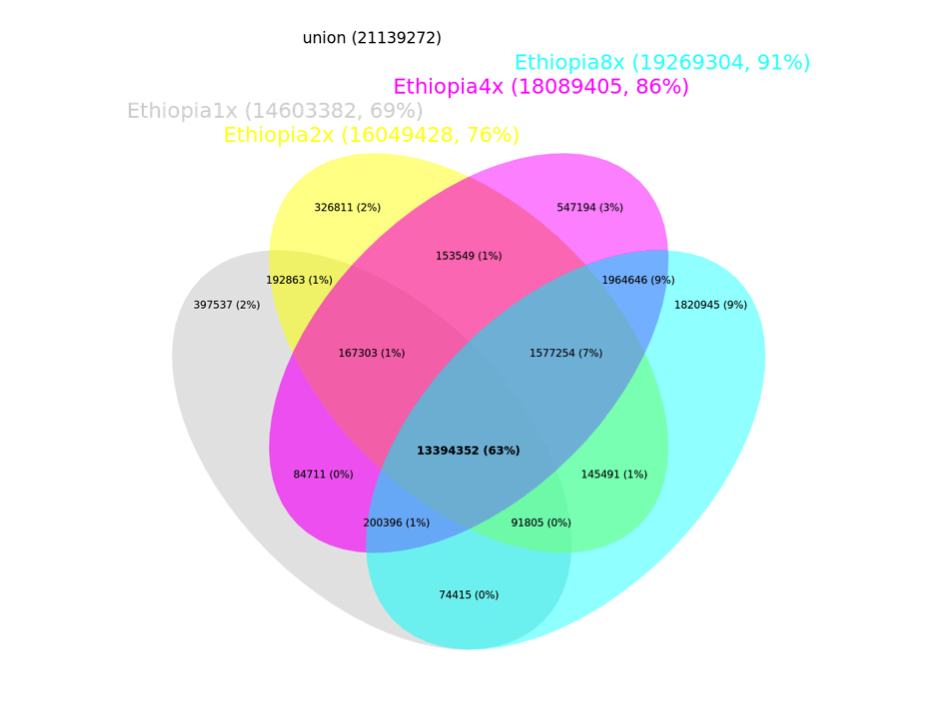
\includegraphics[width=0.45\textwidth]{fig/downsampling_ethiopia_venn.png}
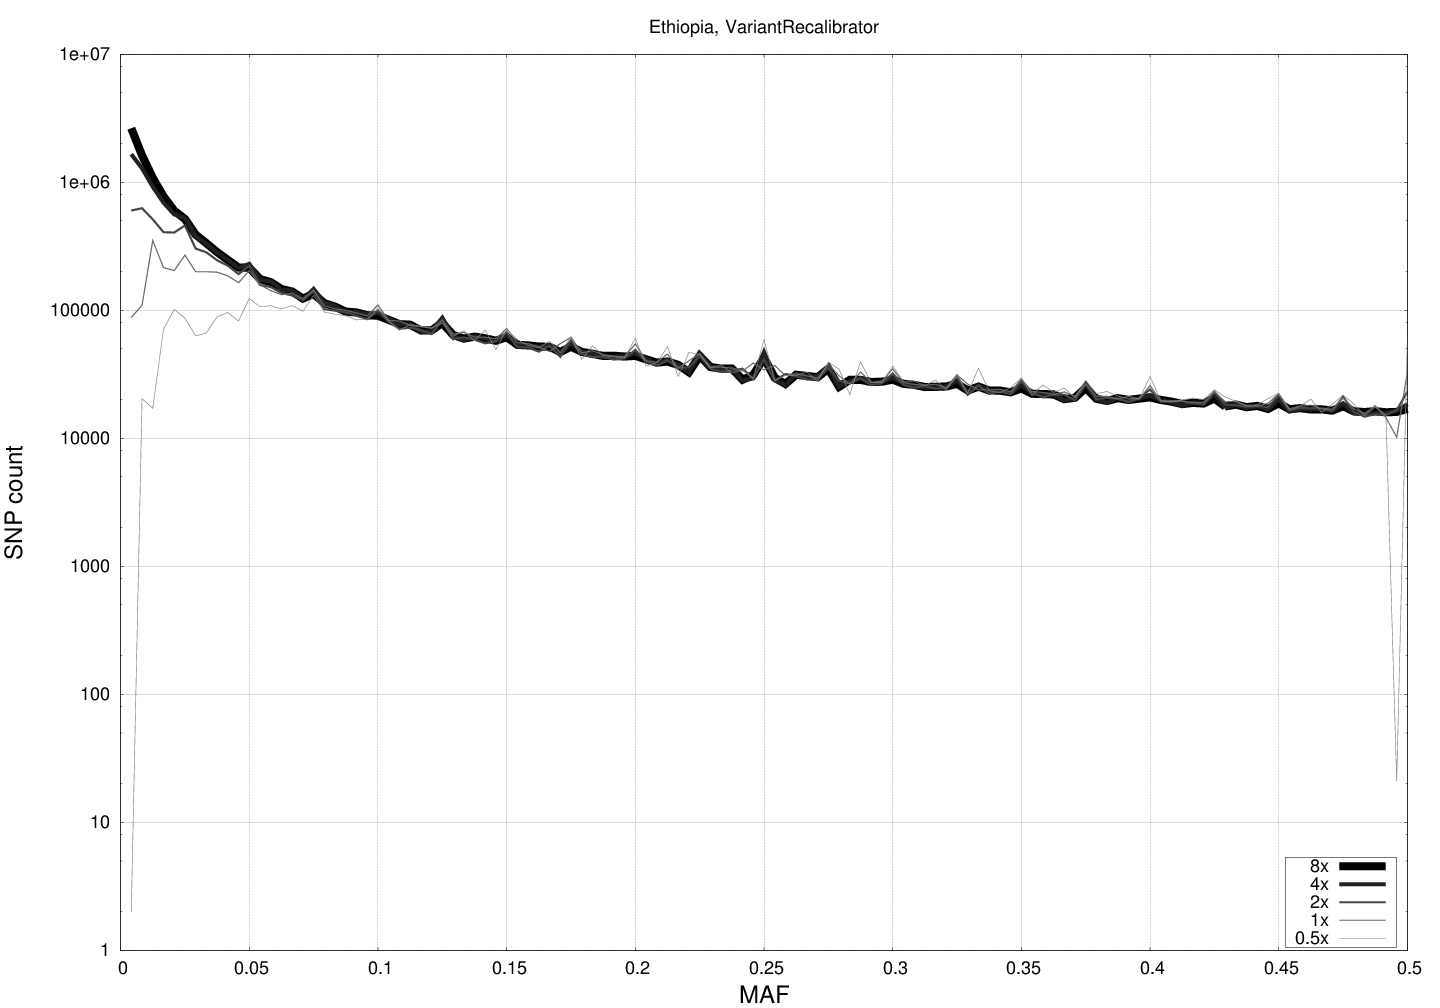
\includegraphics[width=0.45\textwidth]{fig/ethiopia_VR.png}
\caption{Left: Venn diagram showing intersections between call sets at different coverages. Right: \gls{SNP} count in the Ethiopian population at different coverages in different \gls{MAF} bins after calling and filtering of variants with \gls{GATK} UnifiedGenotyper and VariantRecalibrator.\cite{DePristo2011} The y-axis is logarithmic. The ability to call rare variants is impaired at lower coverages.}
\label{fig:downsampling_SNP_count}
\end{figure}
\begin{figure}[htp]
\begin{subfigure}{.3\textwidth}
  \centering
  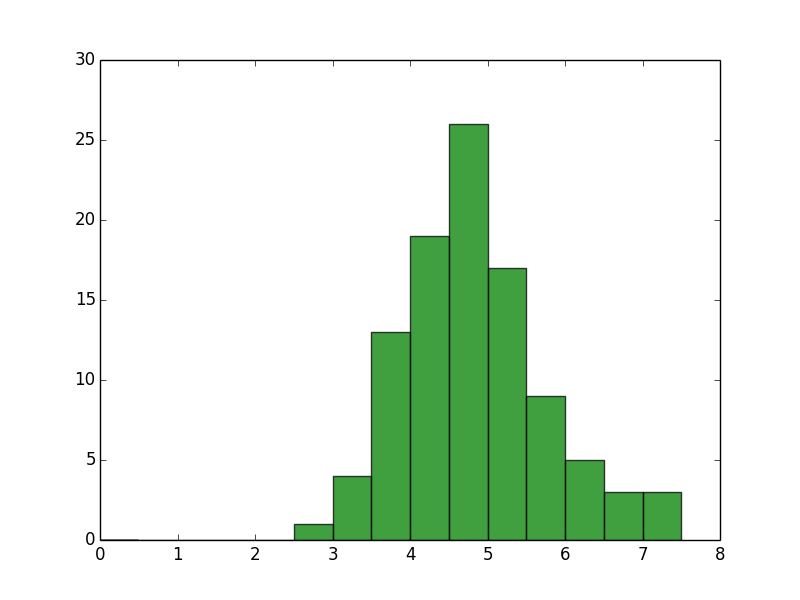
\includegraphics[width=1.0\linewidth]{Chapter2/fig/coverage_baganda.png}
  \caption{Baganda}
\end{subfigure}
\begin{subfigure}{.3\textwidth}
  \centering
  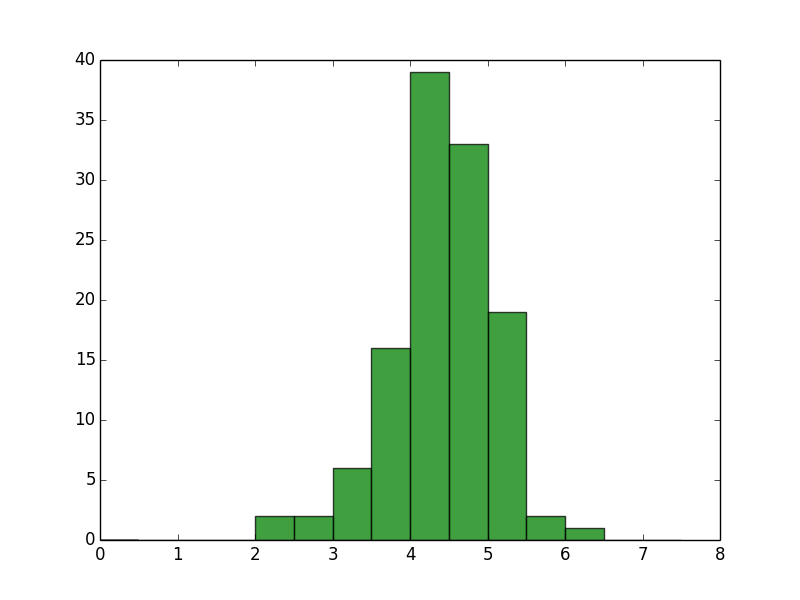
\includegraphics[width=1.0\linewidth]{Chapter2/fig/coverage_ethiopia.png}
  \caption{Ethiopia}
\end{subfigure}
\begin{subfigure}{.3\textwidth}
  \centering
  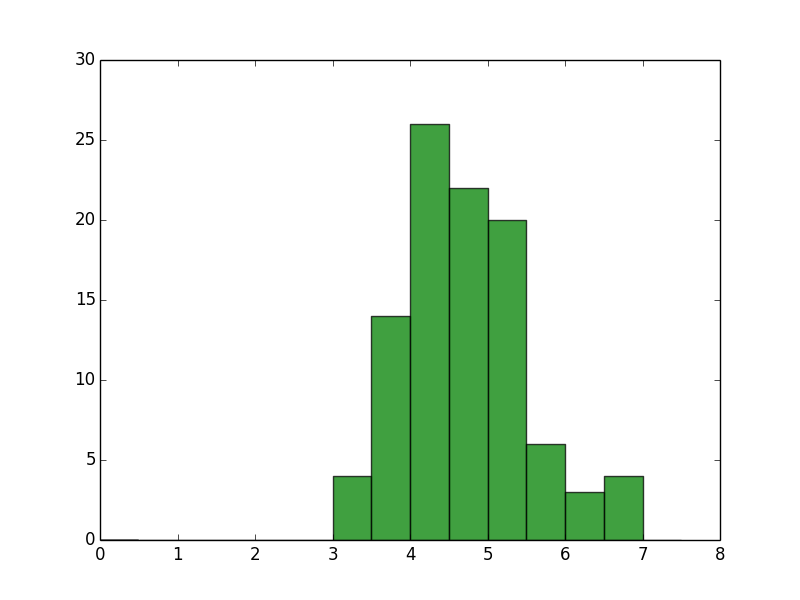
\includegraphics[width=1.0\linewidth]{Chapter2/fig/coverage_zulu.png}
  \caption{Zulu}
\end{subfigure}
\caption{Average depth of coverage in each of the 3 sequenced populations.}
\label{fig:coverage}
\end{figure}
\begin{figure}[htp]
  \centering
  \begin{subfigure}[b]{0.45\textwidth}
    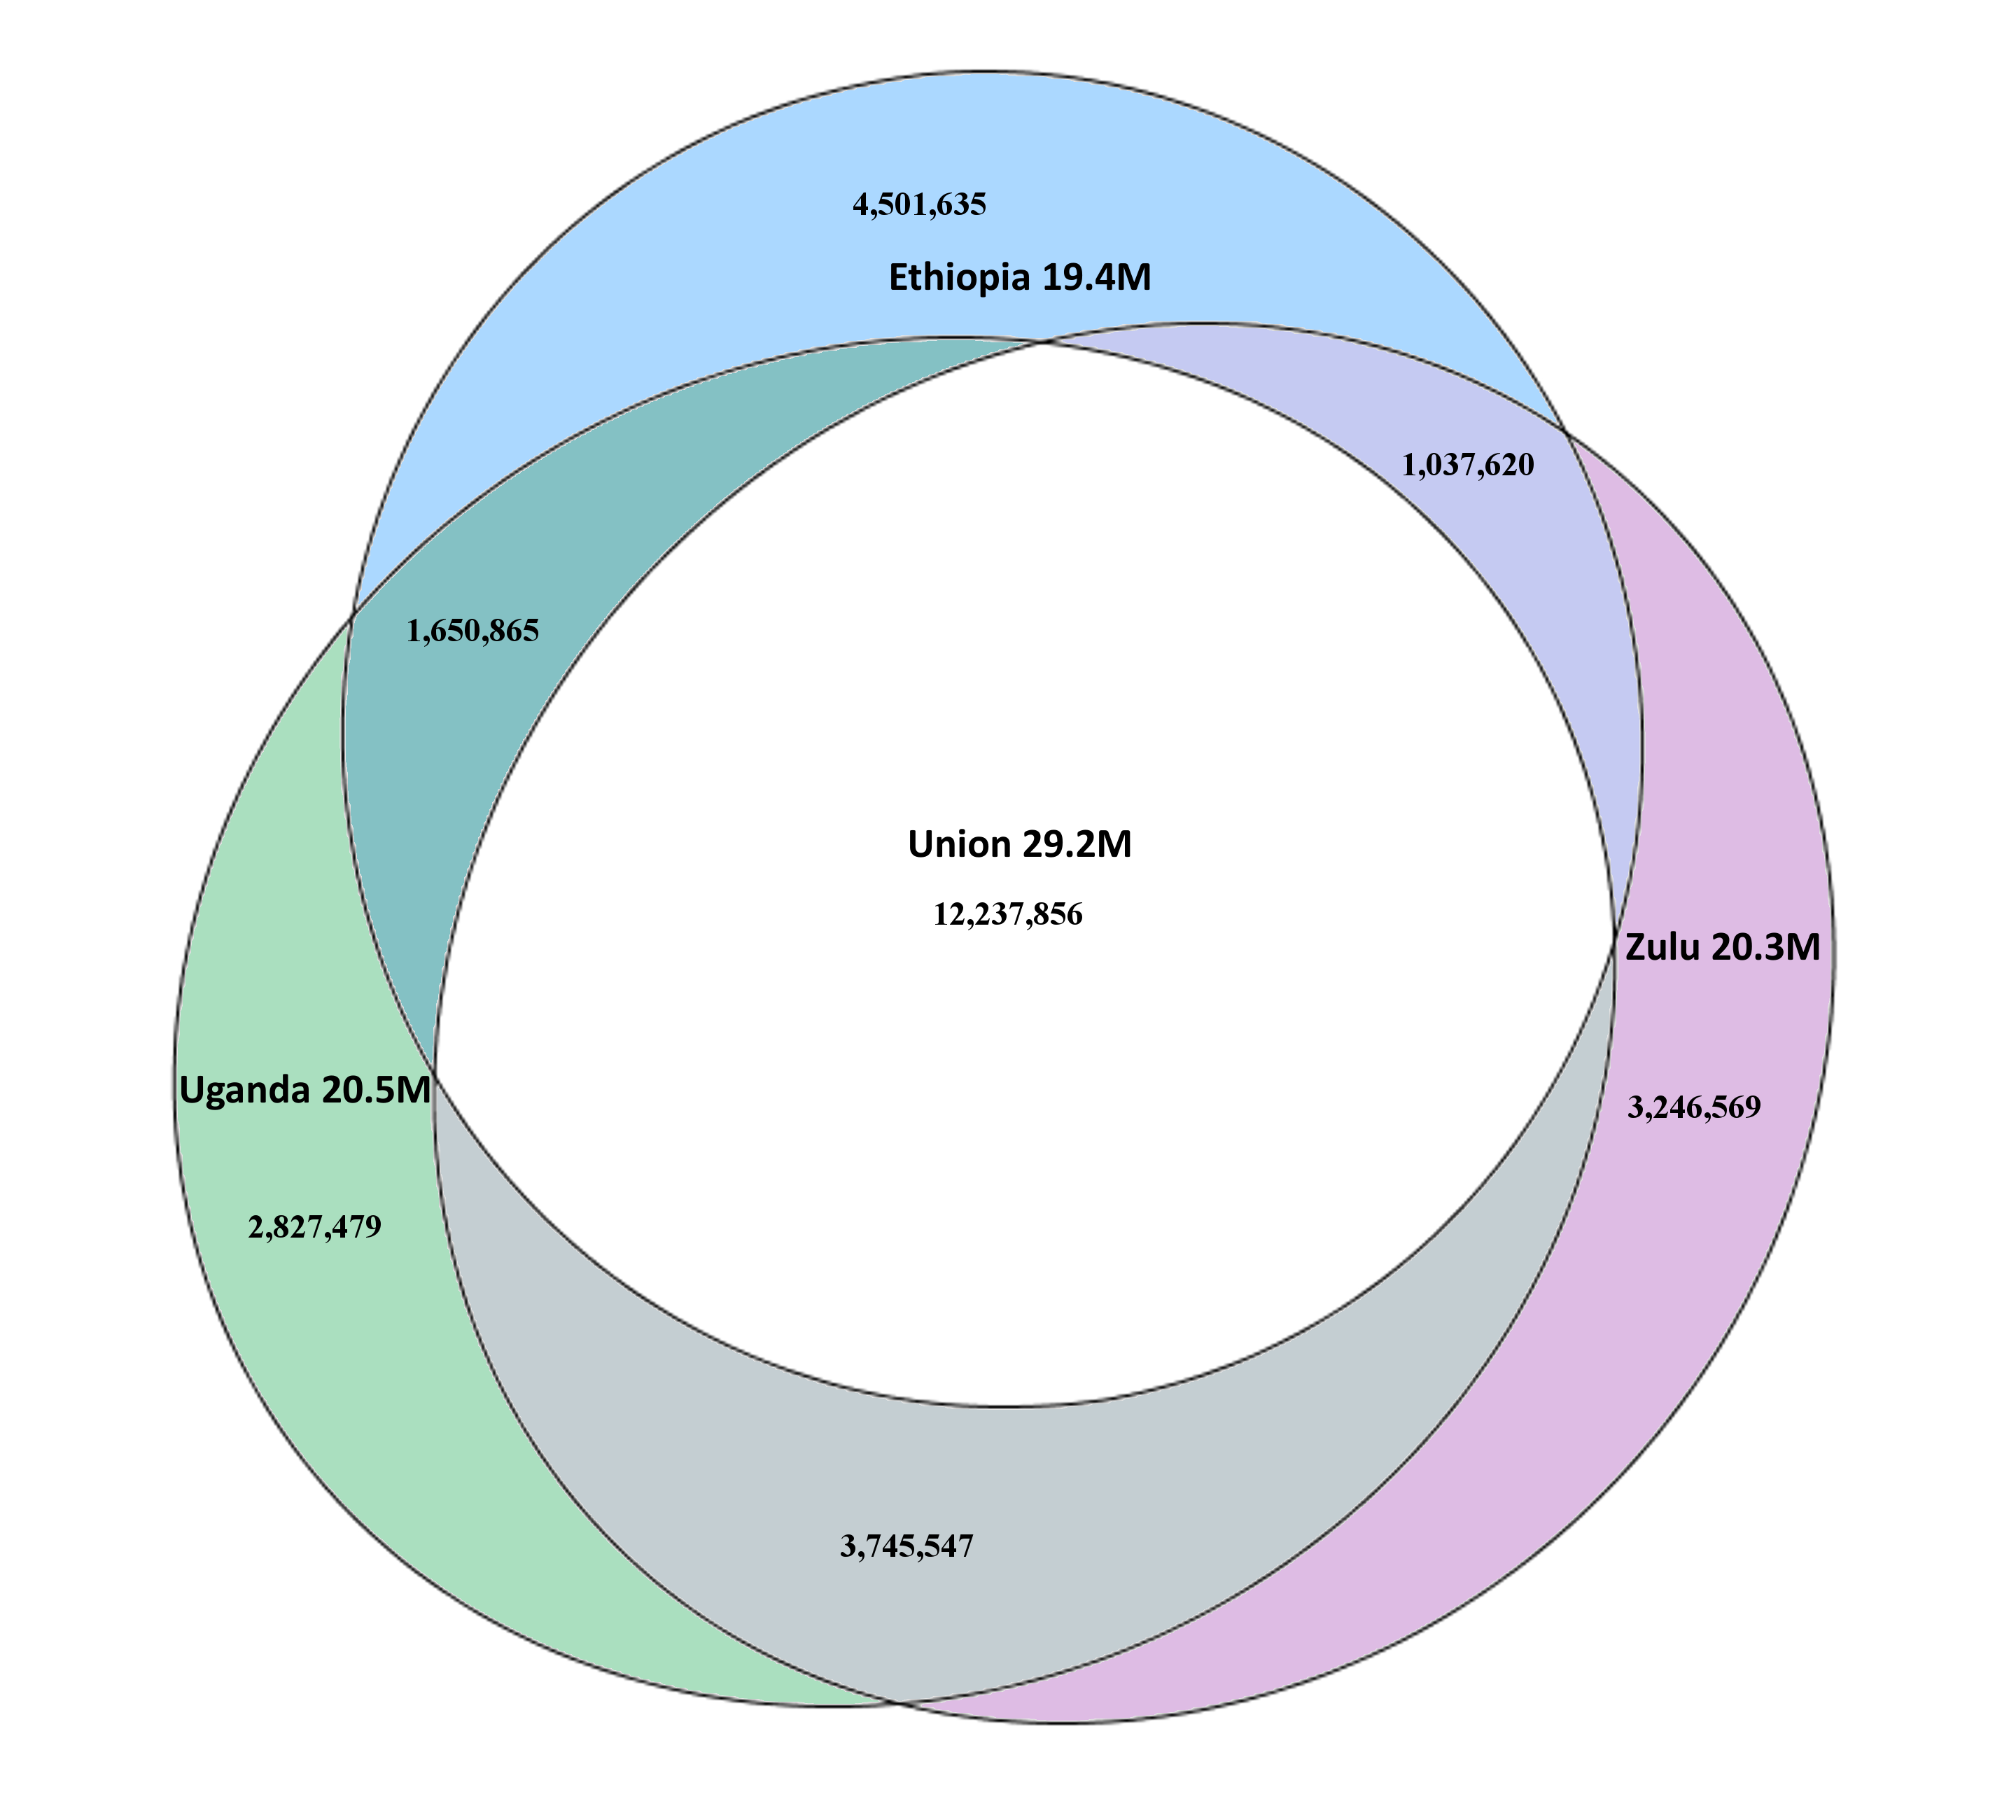
\includegraphics[width=\textwidth]{fig/venn3.png}
    \caption{}
  \end{subfigure}
  \begin{subfigure}[b]{0.45\textwidth}
    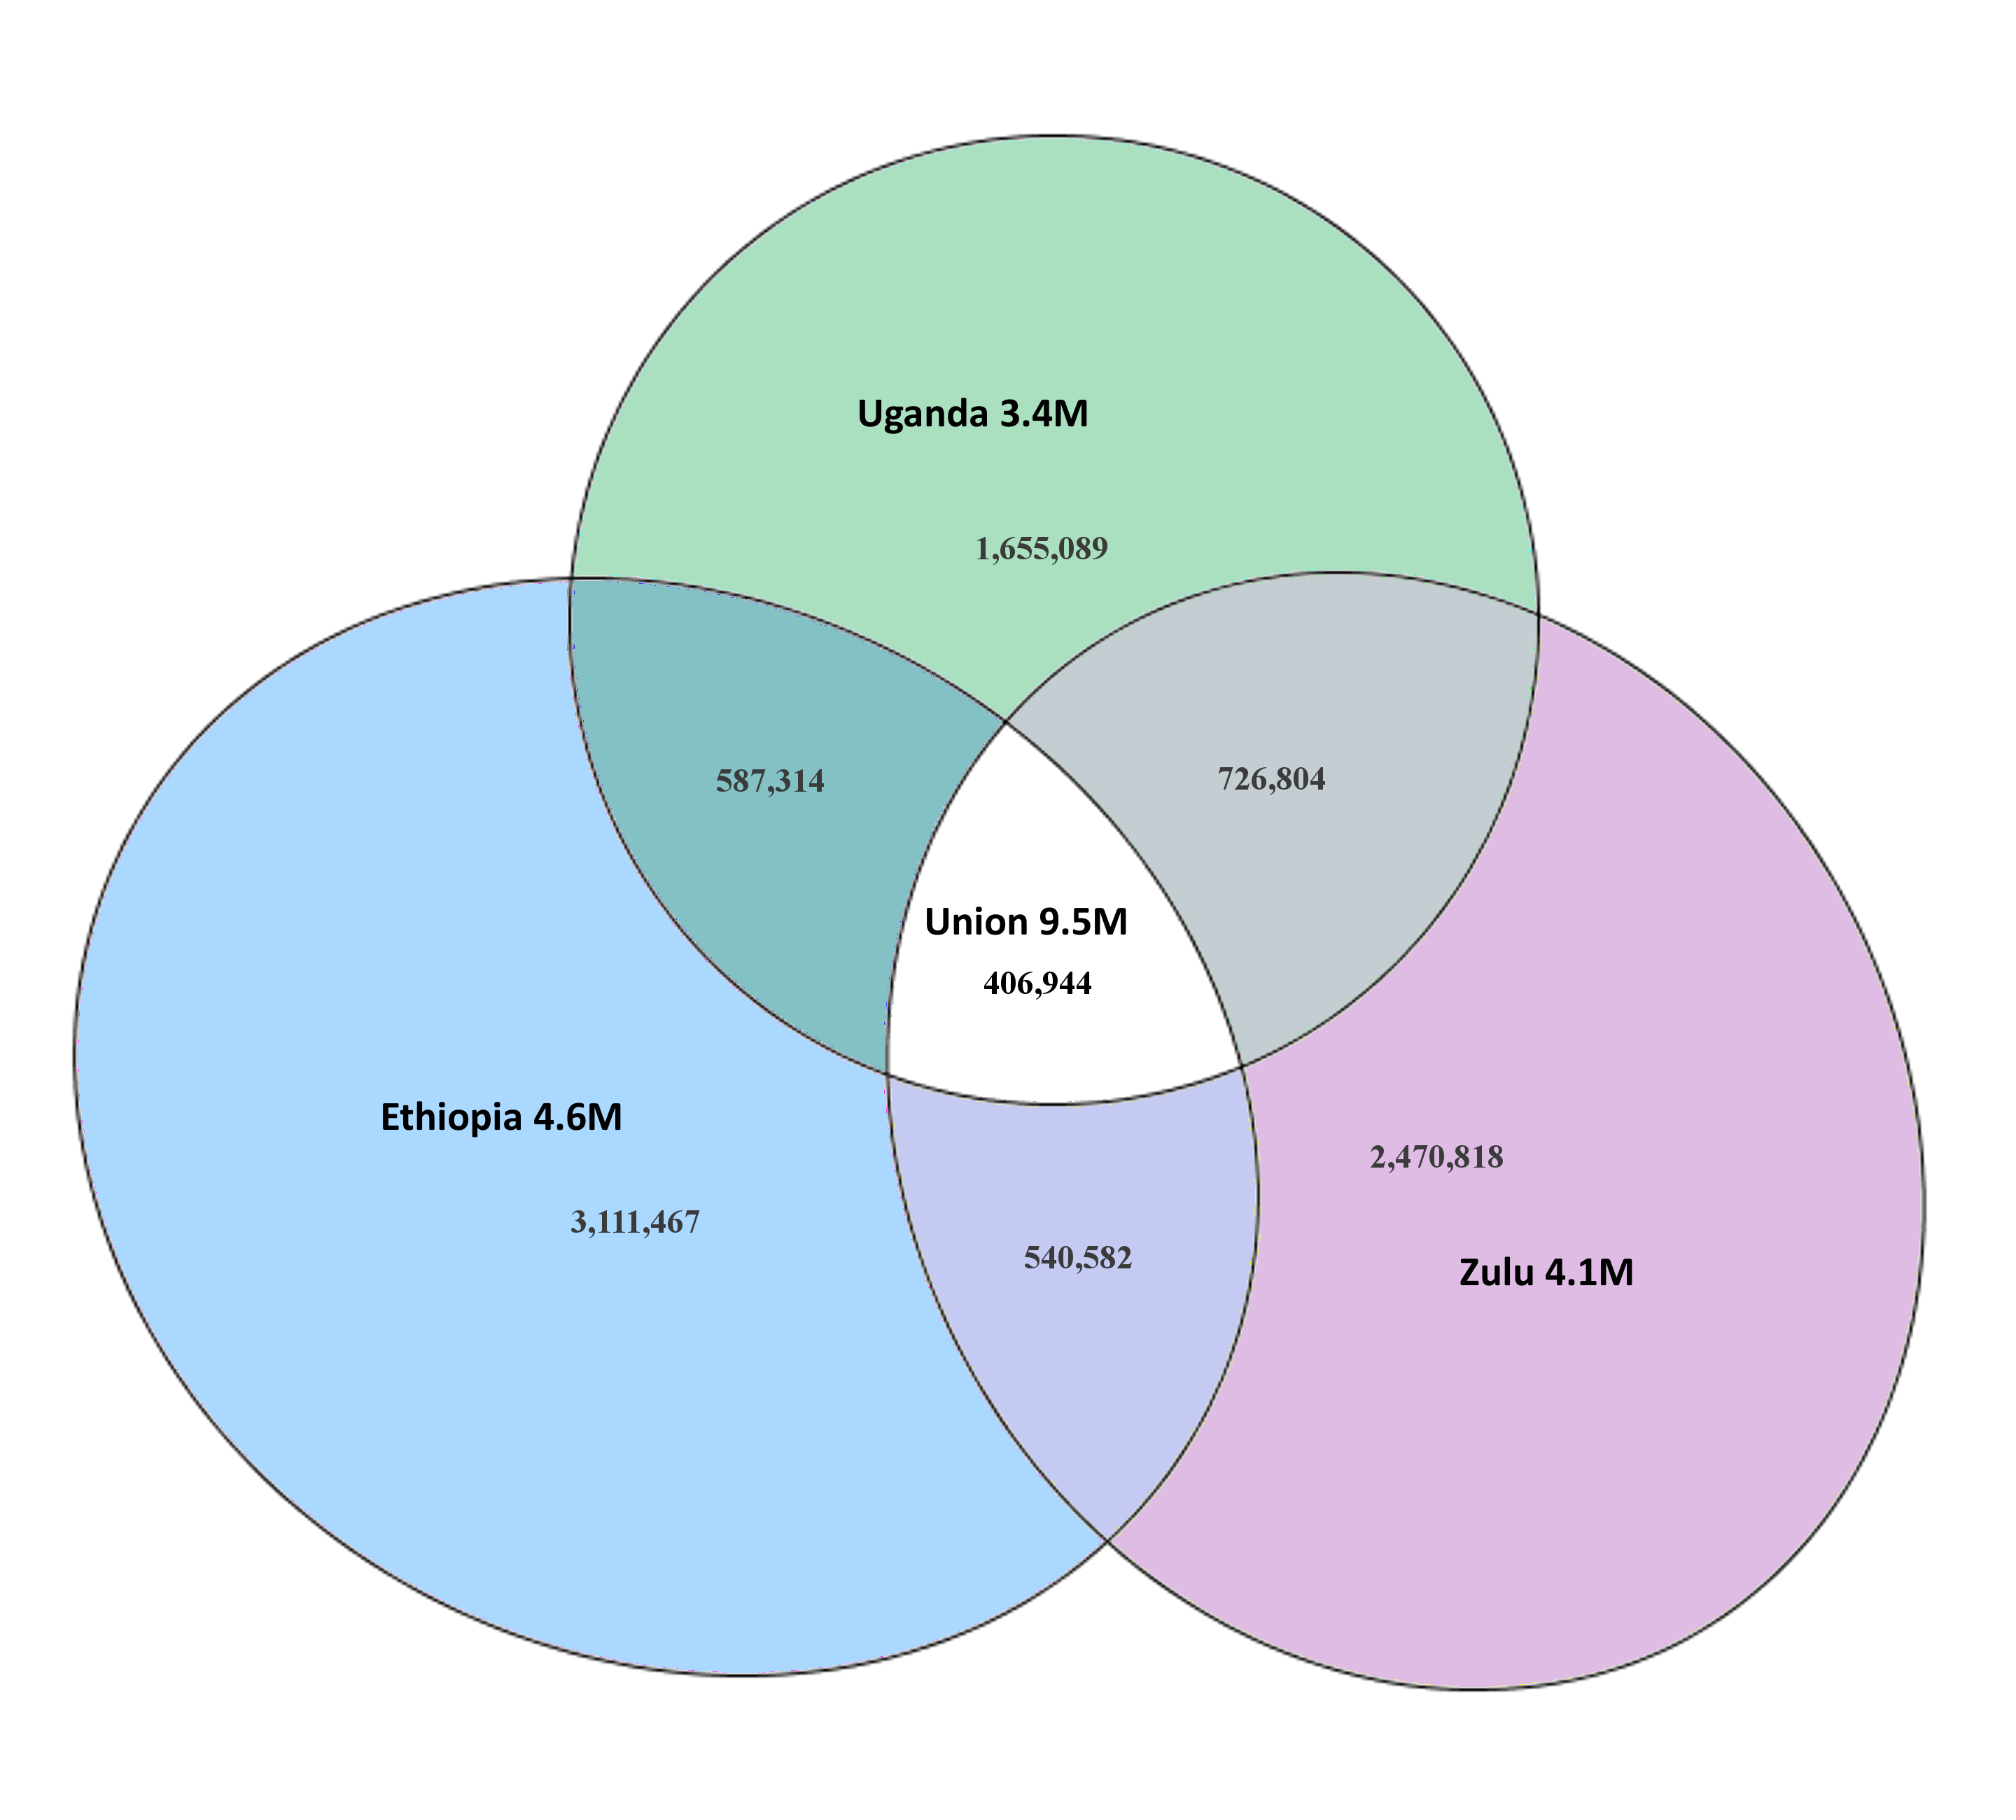
\includegraphics[width=\textwidth]{fig/venn3_complement.png}
    \caption{}
  \end{subfigure}
  \begin{subfigure}[b]{0.45\textwidth}
    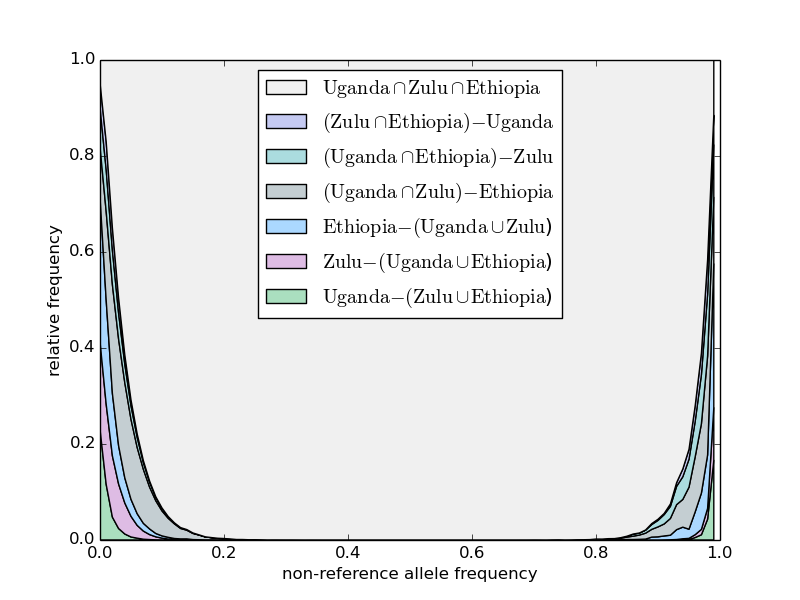
\includegraphics[width=\textwidth]{fig/venn3_stackplot_SNPs.png}
    \caption{}
  \end{subfigure}
  \begin{subfigure}[b]{0.45\textwidth}
    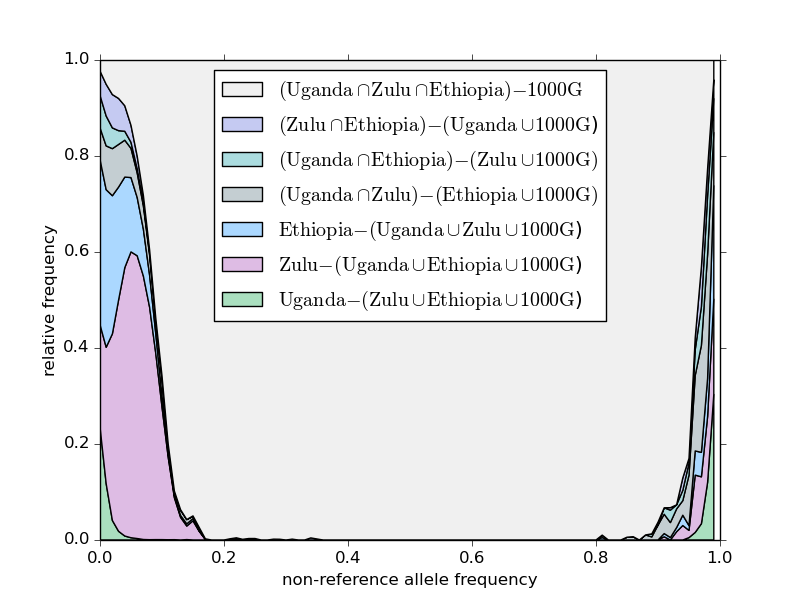
\includegraphics[width=\textwidth]{fig/venn3_stackplot_complement_1000G_SNPs.png}
    \caption{}
  \end{subfigure}
  \caption{Sharing of variants between populations. a) SNP intersection between the 3 sequenced populations subsampled to 100 samples and downsampled to 4x coverage. b) Intersection between the novel variants in the 3 populations; i.e. variants in the relative complement of \gls{1000G} phase 1 with respect to the 3 populations. c) Relative allele frequency spectra for variants in different sets of the Venn diagrams depicted in a and b. The majority of the novel variants with respect to \gls{1000G} are unique to each population. Figures were created with eulerAPE\cite{10.1371/journal.pone.0101717} and matplotlib\cite{Hunter2007}}
  \label{fig:intersection}
\end{figure}
\begin{table}[htp]
\centering
\begin{tabular}{r|rrrr}
{\gls{MAF}} & {4x} & {2x} & {1x} & {0.5x} \\ \hline
0\%                        & 6.7                       & 5.3                       & 4.4                       & 4.0                         \\
(0-1\%{]}                  & 55.1                      & 28.7                      & 14.1                      & 8.0                         \\
(1-2\%{]}                  & 78.9                      & 52.4                      & 29.2                      & 15.0                        \\
(2-5\%{]}                  & 91.0                      & 80.9                      & 61.6                      & 37.2                        \\
(5-10\%{]}                 & 94.2                      & 91.4                      & 87.1                      & 70.5                        \\
(10-20\%{]}                & 95.2                      & 93.6                      & 94.1                      & 91.4                        \\
(20-50\%{]}                & 95.3                      & 95.1                      & 95.6                      & 97.1 \\ \hline
\end{tabular}
\caption[Intersection of \glspl{SNP} between SNP array and sequence data at difference \glspl{AF}.]{Intersection between variants for the 100 Baganda samples on the Omni2.5 platform and the HiSeq2500 platform at different coverages as a percentage of variants on the Omni2.5 platform. Fewer rare SNP array genotyped variants are called at lower coverage.}
\label{tab:downsampling_omni_intersection}
\end{table}

\begin{figure}[htp]
\centering
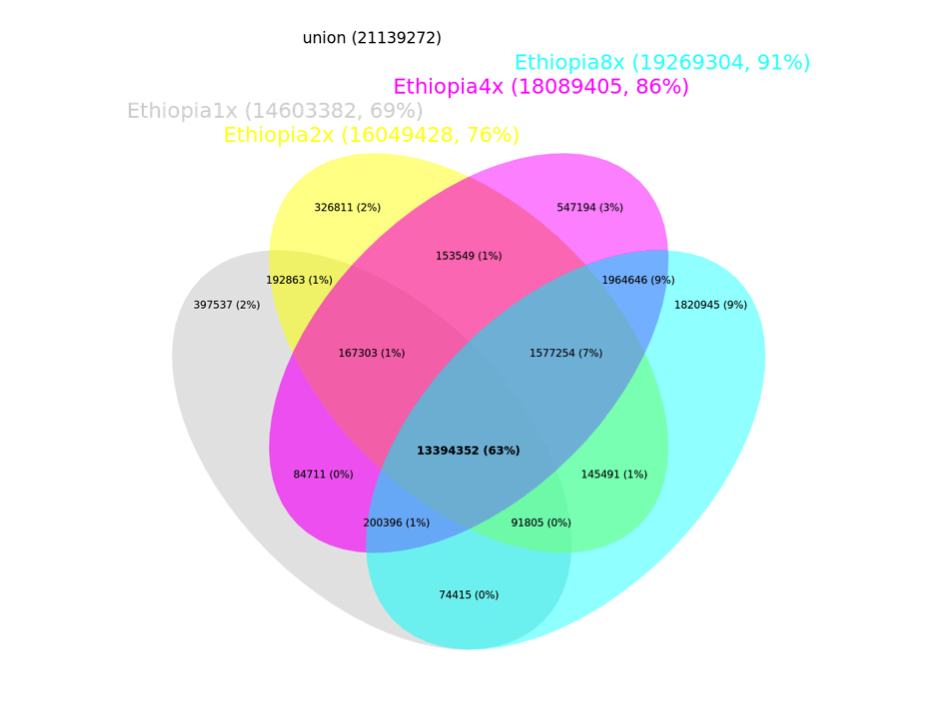
\includegraphics[width=0.45\textwidth]{fig/downsampling_ethiopia_venn.png}
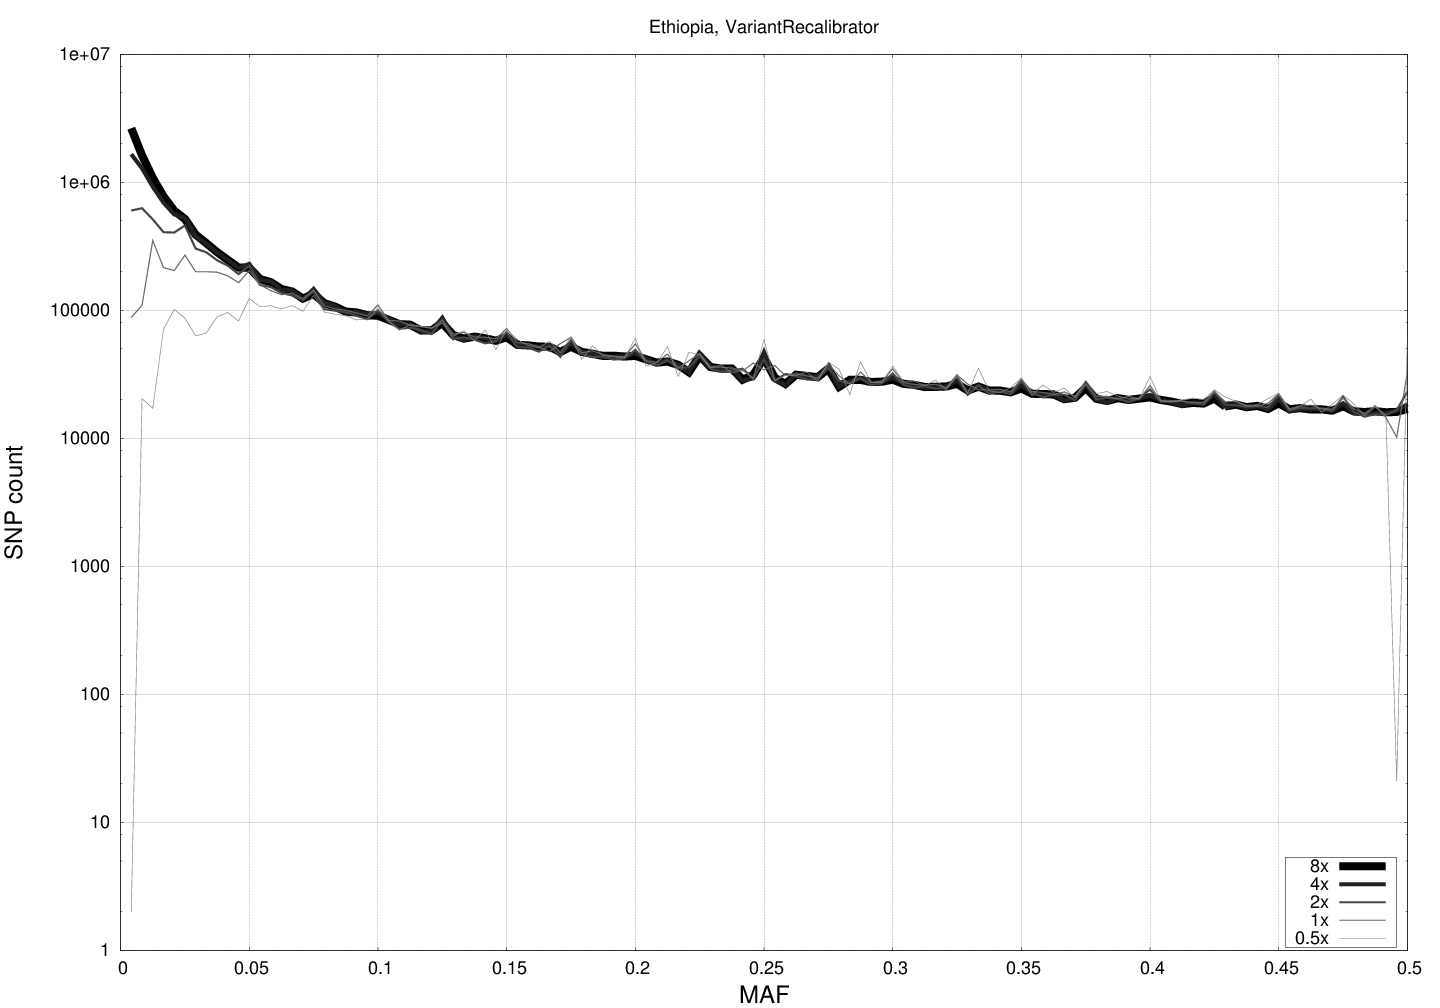
\includegraphics[width=0.45\textwidth]{fig/ethiopia_VR.png}
\caption{Left: Venn diagram showing intersections between call sets at different coverages. Right: \gls{SNP} count in the Ethiopian population at different coverages in different \gls{MAF} bins after calling and filtering of variants with \gls{GATK} UnifiedGenotyper and VariantRecalibrator.\cite{DePristo2011} The y-axis is logarithmic. The ability to call rare variants is impaired at lower coverages.}
\label{fig:downsampling_SNP_count}
\end{figure}

\subsection{Apparent sample size}

Figure - Apparent sample sizes for common, rare and very rare variants without data processing costs. 
Table - Costs associated with acquiring genotypes via two different platforms.